\documentclass[twoside]{iisthesis}
\usepackage[MeX]{polski}
\usepackage[cp1250]{inputenc}
\usepackage{graphicx}
\usepackage{cite}
\usepackage{xcolor}

% definicje kolorow
\definecolor{ciemnoSzary}{rgb}{0.15,0.15,0.15}
\definecolor{szary}{rgb}{0.5,0.5,0.5}
\definecolor{jasnoSzary}{rgb}{0.2,0.2,0.2}
\newcommand\todo[1]{\textcolor{red}{#1}}

\begin{document}

% Zmiana domy�lnych angielskich nazw cz�ci dokumentu na polskie "Rozdzia�y s� w klasie issthesis"
% wst�pnie poprawione mo�e kto� b�dzie zna� lepszy spos�b i wrzuci to do klasy issthesis.cls
\renewcommand{\contentsname}{Spis tre�ci}
\renewcommand{\appendixname}{Dodatek}
\renewcommand{\listfigurename}{Spis ilustracji}
\renewcommand{\listtablename}{Spis tabel}
\renewcommand{\refname}{Bibliografia}
\renewcommand{\abstractname}{Streszczenie}

\title{Predykcja defekt�w na poziomie metod w celu zredukowania wysi�ku zwi�zanego z zapewnieniem jako�ci oprogramowania}
\author{Mateusz Kutyba}
\advisor{dr hab. in�. Lech Madeyski}
\instituteLogo{logos/pwr}
\slowaKluczowe{pierwsze\\drugie\\trzecie}

\date{\number\the\year}

% Wstawienie abstractu pracy
\abstractSH{Bardzo kr�tkie streszczenie w kt�rym powinno si� znale�� om�wienie tematu pracy i poruszanych termin�w. Tekst ten nie mo�e by� zbyt d�ugi.}
\abstractPL{Streszczenie po polsku}
\abstractEN{Abctract in english}

%spis tre�ci
\maketitle
\textpages

%%%%%%%%%%%%%%%%%%%%%%%%%%%%%%%%%%%%%%%%%%%%%%%%%%%%%%%%%%%%
\chapter{Wst�p}
\noindent
	\noindent
T�o: r�ne podej�cia do predykcji defekt�w, potrzeba gromadzenia danych z projekt�w.

Motywacja: istniej�ce modele skupiaj� si� na predykcji na poziomie klas, pakiet�w, plik�w. Przegl�d kodu du�ych projekt�w jest kosztowny.

Dodatkowo gromadzenie danych z projekt�w jest czasoch�onne, wymaga du�o pracy i pobierania projekt�w, potrzeba stworzenia uniwersalnych rozwi�za� s�u��cych do tego celu oraz nastawienie na mo�liwo�� rozszerzania zestawu narz�dzi, kt�re mog� by� ze sob� dowolnie zestawiane




	\section{Cel pracy}
	\noindent
Stworzenie wtyczek do Knime, s�u��cych do wyliczania metryk procesu na podstawie danych z system�w kontroli wersji, zgromadzenie metryk z projekt�w Open Source w repozytorium.

Za�o�enia: wtyczki w �rodowisku Knime, wykorzystanie istniej�cych rozwi�za� platformy DePress, systemy kontroli wersji: git, svn.

Ograniczenia zakresu tematycznego: badanie tylko projekt�w pisanych w Java

	\section{Zwi�zek z innymi pracami}
	\noindent
\begin{itemize}
	\item przegl�d literatury
	\item uzasadnienie, �e nie tworz� czego�, co wcze�niej stworzyli inni
	\item tw�rcze wykorzystanie do�wiadcze� (wynik�w pracy) innych
\end{itemize}





Wst�p Lorem \cite{bramwell2001} ipsum dolor sit amet, consectetur adipiscing elit. Integer odio lectus, egestas sed aliquet ut, semper et tortor. Ut consectetur augue non\cite{padfield2007}metus scelerisque accumsan. Ut quis odio dolor. Suspendisse eu ante ut lorem sagittis lacinia. Mauris elit neque, eleifend eget varius ut, adipiscing sit amet quam. Duis sit amet ullamcorper purus. Aliquam erat volutpat. Donec pharetra massa sed mauris vehicula aliquet eget eu nulla. Etiam non felis metus. Etiam consequat commodo ante. Cras accumsan risus eu enim volutpat quis lobortis risus sagittis. Mauris posuere rutrum ante, at consectetur massa iaculis in.

Duis tristique, sapien et posuere iaculis, sapien lectus ultricies risus, nec placerat risus diam varius arcu. Curabitur eget metus id metus placerat dignissim. Curabitur faucibus est erat, at fermentum lorem. Sed interdum imperdiet erat, vitae dapibus eros feugiat non. Donec sit amet massa nec tortor elementum blandit. Vivamus eget magna odio. Donec hendrerit diam scelerisque arcu porta ut tempus lorem vulputate. Mauris sed tellus in risus bibendum luctus eu et sapien. In et scelerisque purus. Ut vel enim dolor. Proin vitae ipsum odio, nec pretium enim.

Nunc id ligula at felis vestibulum accumsan. Sed molestie erat eu nibh semper tincidunt. In iaculis nisl sed sem dictum ut viverra velit tincidunt. Nunc eros elit, dapibus adipiscing iaculis ut, facilisis sit amet arcu. In blandit, libero vel ornare suscipit, orci eros egestas nisi, ac tincidunt arcu diam non nulla. Mauris auctor, diam ac cursus scelerisque, diam lorem vulputate urna, ut fringilla turpis nunc eget felis. In hac habitasse platea dictumst. Nunc id leo libero. Sed nunc nunc, venenatis sit amet semper mollis, lacinia non purus. Vestibulum id fermentum diam. Suspendisse faucibus massa ac sapien fermentum quis commodo ipsum tempus. Duis sagittis consectetur mi a tincidunt. In quam eros, viverra quis malesuada a, iaculis ac neque. Etiam pharetra, odio varius pharetra interdum, mauris dolor sodales leo, a sagittis enim orci in nulla. Nunc eu quam ligula, nec iaculis tortor.

Sed suscipit interdum vulputate. Nulla vitae accumsan eros. Etiam eu consectetur enim. Duis et erat ut neque vestibulum malesuada. Cras et lectus dolor. Nullam feugiat semper mattis. Suspendisse non justo aliquet risus mattis tristique nec ut orci. Nulla facilisi. Ut bibendum neque sed nibh egestas a cursus mi volutpat. Morbi ac mi a enim tristique cursus. Pellentesque vitae diam massa. Donec dignissim blandit sollicitudin. Nulla dignissim dolor est, ut dictum libero. Ut sagittis tempus semper. Morbi vitae convallis dui. Quisque ut quam massa.

Nunc bibendum orci id nisl posuere sit amet egestas nisl dictum. Cras faucibus hendrerit elit, non suscipit lacus pharetra in. Vivamus eu libero quis risus laoreet egestas. Morbi eleifend aliquet nisi id semper. Cras consequat est id urna malesuada scelerisque. Aliquam tristique, orci vitae suscipit imperdiet, enim magna laoreet leo, in dignissim mi elit vitae lacus. Morbi ut enim vel enim pretium elementum. Maecenas ultricies blandit nisl, eget tincidunt ligula cursus mattis. Fusce et massa non risus euismod gravida at quis quam. Duis sed nibh justo, id semper justo.

Duis tristique, sapien et posuere iaculis, sapien lectus ultricies risus, nec placerat risus diam varius arcu. Curabitur eget metus id metus placerat dignissim. Curabitur faucibus est erat, at fermentum lorem. Sed interdum imperdiet erat, vitae dapibus eros feugiat non. Donec sit amet massa nec tortor elementum blandit. Vivamus eget magna odio. Donec hendrerit diam scelerisque arcu porta ut tempus lorem vulputate. Mauris sed tellus in risus bibendum luctus eu et sapien. In et scelerisque purus. Ut vel enim dolor. Proin vitae ipsum odio, nec pretium enim.

Nunc id ligula at felis vestibulum accumsan. Sed molestie erat eu nibh semper tincidunt. In iaculis nisl sed sem dictum ut viverra velit tincidunt. Nunc eros elit, dapibus adipiscing iaculis ut, facilisis sit amet arcu. In blandit, libero vel ornare suscipit, orci eros egestas nisi, ac tincidunt arcu diam non nulla. Mauris auctor, diam ac cursus scelerisque, diam lorem vulputate urna, ut fringilla turpis nunc eget felis. In hac habitasse platea dictumst. Nunc id leo libero. Sed nunc nunc, venenatis sit amet semper mollis, lacinia non purus. Vestibulum id fermentum diam. Suspendisse faucibus massa ac sapien fermentum quis commodo ipsum tempus. Duis sagittis consectetur mi a tincidunt. In quam eros, viverra quis malesuada a, iaculis ac neque. Etiam pharetra, odio varius pharetra interdum, mauris dolor sodales leo, a sagittis enim orci in nulla. Nunc eu quam ligula, nec iaculis tortor.

Sed suscipit interdum vulputate. Nulla vitae accumsan eros. Etiam eu consectetur enim. Duis et erat ut neque vestibulum malesuada. Cras et lectus dolor. Nullam feugiat semper mattis. Suspendisse non justo aliquet risus mattis tristique nec ut orci. Nulla facilisi. Ut bibendum neque sed nibh egestas a cursus mi volutpat. Morbi ac mi a enim tristique cursus. Pellentesque vitae diam massa. Donec dignissim blandit sollicitudin. Nulla dignissim dolor est, ut dictum libero. Ut sagittis tempus semper. Morbi vitae convallis dui. Quisque ut quam massa.

Nunc bibendum orci id nisl posuere sit amet egestas nisl dictum. Cras faucibus hendrerit elit, non suscipit lacus pharetra in. Vivamus eu libero quis risus laoreet egestas. Morbi eleifend aliquet nisi id semper. Cras consequat est id urna malesuada scelerisque. Aliquam tristique, orci vitae suscipit imperdiet, enim magna laoreet leo, in dignissim mi elit vitae lacus. Morbi ut enim vel enim pretium elementum. Maecenas ultricies blandit nisl, eget tincidunt ligula cursus mattis. Fusce et massa non risus euismod gravida at quis quam. Duis sed nibh justo, id semper justo.

Duis tristique, sapien et posuere iaculis, sapien lectus ultricies risus, nec placerat risus diam varius arcu. Curabitur eget metus id metus placerat dignissim. Curabitur faucibus est erat, at fermentum lorem. Sed interdum imperdiet erat, vitae dapibus eros feugiat non. Donec sit amet massa nec tortor elementum blandit. Vivamus eget magna odio. Donec hendrerit diam scelerisque arcu porta ut tempus lorem vulputate. Mauris sed tellus in risus bibendum luctus eu et sapien. In et scelerisque purus. Ut vel enim dolor. Proin vitae ipsum odio, nec pretium enim.

Nunc id ligula at felis vestibulum accumsan. Sed molestie erat eu nibh semper tincidunt. In iaculis nisl sed sem dictum ut viverra velit tincidunt. Nunc eros elit, dapibus adipiscing iaculis ut, facilisis sit amet arcu. In blandit, libero vel ornare suscipit, orci eros egestas nisi, ac tincidunt arcu diam non nulla. Mauris auctor, diam ac cursus scelerisque, diam lorem vulputate urna, ut fringilla turpis nunc eget felis. In hac habitasse platea dictumst. Nunc id leo libero. Sed nunc nunc, venenatis sit amet semper mollis, lacinia non purus. Vestibulum id fermentum diam. Suspendisse faucibus massa ac sapien fermentum quis commodo ipsum tempus. Duis sagittis consectetur mi a tincidunt. In quam eros, viverra quis malesuada a, iaculis ac neque. Etiam pharetra, odio varius pharetra interdum, mauris dolor sodales leo, a sagittis enim orci in nulla. Nunc eu quam ligula, nec iaculis tortor.

Sed suscipit interdum vulputate. Nulla vitae accumsan eros. Etiam eu consectetur enim. Duis et erat ut neque vestibulum malesuada. Cras et lectus dolor. Nullam feugiat semper mattis. Suspendisse non justo aliquet risus mattis tristique nec ut orci. Nulla facilisi. Ut bibendum neque sed nibh egestas a cursus mi volutpat. Morbi ac mi a enim tristique cursus. Pellentesque vitae diam massa. Donec dignissim blandit sollicitudin. Nulla dignissim dolor est, ut dictum libero. Ut sagittis tempus semper. Morbi vitae convallis dui. Quisque ut quam massa.

Nunc bibendum orci id nisl posuere sit amet egestas nisl dictum. Cras faucibus hendrerit elit, non suscipit lacus pharetra in. Vivamus eu libero quis risus laoreet egestas. Morbi eleifend aliquet nisi id semper. Cras consequat est id urna malesuada scelerisque. Aliquam tristique, orci vitae suscipit imperdiet, enim magna laoreet leo, in dignissim mi elit vitae lacus. Morbi ut enim vel enim pretium elementum. Maecenas ultricies blandit nisl, eget tincidunt ligula cursus mattis. Fusce et massa non risus euismod gravida at quis quam. Duis sed nibh justo, id semper justo.
Duis tristique, sapien et posuere iaculis, sapien lectus ultricies risus, nec placerat risus diam varius arcu. Curabitur eget metus id metus placerat dignissim. Curabitur faucibus est erat, at fermentum lorem. Sed interdum imperdiet erat, vitae dapibus eros feugiat non. Donec sit amet massa nec tortor elementum blandit. Vivamus eget magna odio. Donec hendrerit diam scelerisque arcu porta ut tempus lorem vulputate. Mauris sed tellus in risus bibendum luctus eu et sapien. In et scelerisque purus. Ut vel enim dolor. Proin vitae ipsum odio, nec pretium enim.

Nunc id ligula at felis vestibulum accumsan. Sed molestie erat eu nibh semper tincidunt. In iaculis nisl sed sem dictum ut viverra velit tincidunt. Nunc eros elit, dapibus adipiscing iaculis ut, facilisis sit amet arcu. In blandit, libero vel ornare suscipit, orci eros egestas nisi, ac tincidunt arcu diam non nulla. Mauris auctor, diam ac cursus scelerisque, diam lorem vulputate urna, ut fringilla turpis nunc eget felis. In hac habitasse platea dictumst. Nunc id leo libero. Sed nunc nunc, venenatis sit amet semper mollis, lacinia non purus. Vestibulum id fermentum diam. Suspendisse faucibus massa ac sapien fermentum quis commodo ipsum tempus. Duis sagittis consectetur mi a tincidunt. In quam eros, viverra quis malesuada a, iaculis ac neque. Etiam pharetra, odio varius pharetra interdum, mauris dolor sodales leo, a sagittis enim orci in nulla. Nunc eu quam ligula, nec iaculis tortor.

Sed suscipit interdum vulputate. Nulla vitae accumsan eros. Etiam eu consectetur enim. Duis et erat ut neque vestibulum malesuada. Cras et lectus dolor. Nullam feugiat semper mattis. Suspendisse non justo aliquet risus mattis tristique nec ut orci. Nulla facilisi. Ut bibendum neque sed nibh egestas a cursus mi volutpat. Morbi ac mi a enim tristique cursus. Pellentesque vitae diam massa. Donec dignissim blandit sollicitudin. Nulla dignissim dolor est, ut dictum libero. Ut sagittis tempus semper. Morbi vitae convallis dui. Quisque ut quam massa.

Nunc bibendum orci id nisl posuere sit amet egestas nisl dictum. Cras faucibus hendrerit elit, non suscipit lacus pharetra in. Vivamus eu libero quis risus laoreet egestas. Morbi eleifend aliquet nisi id semper. Cras consequat est id urna malesuada scelerisque. Aliquam tristique, orci vitae suscipit imperdiet, enim magna laoreet leo, in dignissim mi elit vitae lacus. Morbi ut enim vel enim pretium elementum. Maecenas ultricies blandit nisl, eget tincidunt ligula cursus mattis. Fusce et massa non risus euismod gravida at quis quam. Duis sed nibh justo, id semper justo.
Duis tristique, sapien et posuere iaculis, sapien lectus ultricies risus, nec placerat risus diam varius arcu. Curabitur eget metus id metus placerat dignissim. Curabitur faucibus est erat, at fermentum lorem. Sed interdum imperdiet erat, vitae dapibus eros feugiat non. Donec sit amet massa nec tortor elementum blandit. Vivamus eget magna odio. Donec hendrerit diam scelerisque arcu porta ut tempus lorem vulputate. Mauris sed tellus in risus bibendum luctus eu et sapien. In et scelerisque purus. Ut vel enim dolor. Proin vitae ipsum odio, nec pretium enim.

Nunc id ligula at felis vestibulum accumsan. Sed molestie erat eu nibh semper tincidunt. In iaculis nisl sed sem dictum ut viverra velit tincidunt. Nunc eros elit, dapibus adipiscing iaculis ut, facilisis sit amet arcu. In blandit, libero vel ornare suscipit, orci eros egestas nisi, ac tincidunt arcu diam non nulla. Mauris auctor, diam ac cursus scelerisque, diam lorem vulputate urna, ut fringilla turpis nunc eget felis. In hac habitasse platea dictumst. Nunc id leo libero. Sed nunc nunc, venenatis sit amet semper mollis, lacinia non purus. Vestibulum id fermentum diam. Suspendisse faucibus massa ac sapien fermentum quis commodo ipsum tempus. Duis sagittis consectetur mi a tincidunt. In quam eros, viverra quis malesuada a, iaculis ac neque. Etiam pharetra, odio varius pharetra interdum, mauris dolor sodales leo, a sagittis enim orci in nulla. Nunc eu quam ligula, nec iaculis tortor.

Sed suscipit interdum vulputate. Nulla vitae accumsan eros. Etiam eu consectetur enim. Duis et erat ut neque vestibulum malesuada. Cras et lectus dolor. Nullam feugiat semper mattis. Suspendisse non justo aliquet risus mattis tristique nec ut orci. Nulla facilisi. Ut bibendum neque sed nibh egestas a cursus mi volutpat. Morbi ac mi a enim tristique cursus. Pellentesque vitae diam massa. Donec dignissim blandit sollicitudin. Nulla dignissim dolor est, ut dictum libero. Ut sagittis tempus semper. Morbi vitae convallis dui. Quisque ut quam massa.

Nunc bibendum orci id nisl posuere sit amet egestas nisl dictum. Cras faucibus hendrerit elit, non suscipit lacus pharetra in. Vivamus eu libero quis risus laoreet egestas. Morbi eleifend aliquet nisi id semper. Cras consequat est id urna malesuada scelerisque. Aliquam tristique, orci vitae suscipit imperdiet, enim magna laoreet leo, in dignissim mi elit vitae lacus. Morbi ut enim vel enim pretium elementum. Maecenas ultricies blandit nisl, eget tincidunt ligula cursus mattis. Fusce et massa non risus euismod gravida at quis quam. Duis sed nibh justo, id semper justo.
Duis tristique, sapien et posuere iaculis, sapien lectus ultricies risus, nec placerat risus diam varius arcu. Curabitur eget metus id metus placerat dignissim. Curabitur faucibus est erat, at fermentum lorem. Sed interdum imperdiet erat, vitae dapibus eros feugiat non. Donec sit amet massa nec tortor elementum blandit. Vivamus eget magna odio. Donec hendrerit diam scelerisque arcu porta ut tempus lorem vulputate. Mauris sed tellus in risus bibendum luctus eu et sapien. In et scelerisque purus. Ut vel enim dolor. Proin vitae ipsum odio, nec pretium enim.

Nunc id ligula at felis vestibulum accumsan. Sed molestie erat eu nibh semper tincidunt. In iaculis nisl sed sem dictum ut viverra velit tincidunt. Nunc eros elit, dapibus adipiscing iaculis ut, facilisis sit amet arcu. In blandit, libero vel ornare suscipit, orci eros egestas nisi, ac tincidunt arcu diam non nulla. Mauris auctor, diam ac cursus scelerisque, diam lorem vulputate urna, ut fringilla turpis nunc eget felis. In hac habitasse platea dictumst. Nunc id leo libero. Sed nunc nunc, venenatis sit amet semper mollis, lacinia non purus. Vestibulum id fermentum diam. Suspendisse faucibus massa ac sapien fermentum quis commodo ipsum tempus. Duis sagittis consectetur mi a tincidunt. In quam eros, viverra quis malesuada a, iaculis ac neque. Etiam pharetra, odio varius pharetra interdum, mauris dolor sodales leo, a sagittis enim orci in nulla. Nunc eu quam ligula, nec iaculis tortor.

Sed suscipit interdum vulputate. Nulla vitae accumsan eros. Etiam eu consectetur enim. Duis et erat ut neque vestibulum malesuada. Cras et lectus dolor. Nullam feugiat semper mattis. Suspendisse non justo aliquet risus mattis tristique nec ut orci. Nulla facilisi. Ut bibendum neque sed nibh egestas a cursus mi volutpat. Morbi ac mi a enim tristique cursus. Pellentesque vitae diam massa. Donec dignissim blandit sollicitudin. Nulla dignissim dolor est, ut dictum libero. Ut sagittis tempus semper. Morbi vitae convallis dui. Quisque ut quam massa.

Nunc bibendum orci id nisl posuere sit amet egestas nisl dictum. Cras faucibus hendrerit elit, non suscipit lacus pharetra in. Vivamus eu libero quis risus laoreet egestas. Morbi eleifend aliquet nisi id semper. Cras consequat est id urna malesuada scelerisque. Aliquam tristique, orci vitae suscipit imperdiet, enim magna laoreet leo, in dignissim mi elit vitae lacus. Morbi ut enim vel enim pretium elementum. Maecenas ultricies blandit nisl, eget tincidunt ligula cursus mattis. Fusce et massa non risus euismod gravida at quis quam. Duis sed nibh justo, id semper justo.

%%%%%%%%%%%%%%%%%%%%%%%%%%%%%%%%%%%%%%%%%%%%%%%%%%%%%%%%%%%%
\chapter{Wprowadzenie}
\noindent
%%%%%%%%%%%%%%%%%%%%%%%%%%%%%%%%%%%%%%%%%%%%%%%%%%%%%%%%%%%%
%%%%%%%%%%%%%%%%%%%%%%%%%%%%%%%%%%%%%%%%%%%%%%%%%%%%%%%%%%%%
\section{Rola metryk w in�ynierii oprogramowania}
\label{rola-metryk}

\noindent Norma IEEE 1061-1998 \cite{749159} definiuje metryk� jako ``funkcj� odwzorowuj�c� jednostk� oprogramowania w warto�� liczbow�. Ta wyliczona warto�� jest interpretowalna jako stopie� spe�nienia pewnej w�asno�ci jako�ci jednostki oprogramowania."

W in�ynierii oprogramowania metryki s� wykorzystywane we wszystkich fazach procesu wytwarzania oprogramowania. Pozwalaj� na por�wnywanie ze sob� r�nych element�w lub r�nych projekt�w poniewa� s� danymi liczbowymi. W fazie projektowania mog� s�u�y� m.in. do szacowania nak�adu pracy potrzebnego do realizacji projektu. W fazie produkcji i test�w do mierzenia jako�ci aplikacji, wydajno�ci pracy czy z�o�ono�ci programu.

Metryki mo�na podzieli� wed�ug r�nych kryeri�w. Ze wzgl�du na typ artefaktu jaki opisuj� dzieli si� je na:
\begin{itemize}
	\item Metryki produktu (inaczej metryki kodu �r�d�owego). S� bezpo�rednio wyliczane z kodu �r�d�owego programu. Przyk�adem takich metryk s�:
	\begin{itemize}
		\item Zestaw metryk CK \cite{chidamber1994metrics}, do kt�rego nale��:
		\begin{itemize}
			\item u�rednione metody na klas� (ang. \textit{Weighted Methods per Class}, WMC),
			\item g��boko�� drzewa dziedziczenia (ang. \textit{Depth of Inheritance Tree}, DIT),
			\item liczba dzieci (ang. \textit{Number of Children}, NOC),
			\item zale�no�� mi�dzy obiektami (ang. \textit{Coupling Between Objects}, CBO),
			\item odpowiedzialno�� danej klasy (ang. \textit{Response For a Class}, RFC),
			\item brak sp�jno�ci metod (ang. \textit{Lack of Cohesion of Methods}, LCOM).
		\end{itemize}
		\item OO --- metryki obiektowe, np.:
		\begin{itemize}
			\item liczba atrybut�w (ang. \textit{Number of attributes}, NOA),
			\item liczba metod (ang. \textit{Number of methods}, NOM),
			\item liczba dziedziczonych metod (ang. \textit{Number of methods inherited}, NOMI).
		\end{itemize}
		\item LOC --- liczba linii kodu.
	\end{itemize}
	\item Metryki procesu (inaczej metryki zmian). Okre�laj� zmienno�� atrybutu w czasie. Oblicza si� je dla zadanych przedzia��w czasowych. Niezb�dna do ich obliczenia jest historia projektu, kt�r� mo�na uzyska� dzi�ki systemom kontroli wersji (jak SVN czy Git). Przyk�ady metryk procesu:
		\begin{itemize}
			\item liczba modyfikacji (rewizji) pliku (ang. \textit{Number of Revisions}, NR),
			\item liczba autor�w zmieniaj�cych plik (ang. \textit{Number of Distinct Commiters}, NDC),
			\item liczba zmienionych linii kodu (ang. \textit{Number of Modi?ed Lines}, NML),
			\item wiek pliku (ang. \textit{Age}, AGE),
			\item liczba refaktoryzacji pliku (ang. \textit{(Number of Refactorings}, NREF),
			\item liczba dodanych (usuni�tych, zmienionych) metod,
			\item liczba dodanych (usuni�tych, zmienionych) atrybut�w.
		\end{itemize}
\end{itemize}

Dodatkowo mo�na podzieli� metryki z uwagi na cel pomiaru \cite{gorski2000inzynieria}:
\begin{itemize}
	\item metryki z�o�ono�ci,
	\item metryki szacowania nak�adu,
	\item metryki funkcjonalno�ci.
\end{itemize}


Model predykcji defekt�w to narz�dzie, kt�re na podstawie warto�ci metryk danego projektu dokonuje wskazania defekt�w znajduj�cych si� w tym projekcie. Aby poprawnie zinterpretowa� wskazania dostarczane przez model predykcji defekt�w zdefiniowa� defekt. Norma 982.2 IEEE/ANSI \cite{26479} definiuje defekt jako anomali� w produkcie, kt�ra mo�e by�:
\begin{itemize}
	\item zaniechaniami i niedoskona�o�ciami znalezionymi podczas wczesnych faz cyklu �ycia oraz
	\item b��dami zawartymi w oprogramowaniu wystarczaj�co dojrza�ym do testowania lub dzia�ania.
\end{itemize}

Istniej�ce badania wykaza�y, �e metryki procesu przewy�szy�y metryki produktu w kontek�cie budowania modeli predykcji defekt�w \cite{giger2012method, kamei2010revisiting, mende2009revisiting, ferzund2009empirical}. Z tego powodu w dalszej cz�ci pracy zrezygnowano z wykorzystania metryk produktu, bior�c pod uwag� jedynie metryki procesu.



%Likewise, Kamei et al. (2010) revisited common findings in defect prediction when
%using effort-aware performance measurements. One finding that they confirmed is
%that process metrics (i.e., extracted from the version control system or the defect
%database) still perform better than product metrics (i.e., metrics of the software
%system itself).
%	Kamei Y, Matsumoto S, Monden A, Matsumoto K-i, Adams B, Hassan AE (2010) Revisit-
%	ing common bug prediction findings using effort aware models. In: Proceedings of the 26th
%	IEEE international conference on software maintenance (ICSM 2010). IEEE CS, Washington,
%	pp 1�10
%These findings corroborate those of Mende and Koschke (2009), and of Kamei
%et al. (2010), which found that product metrics were outperformed by process metrics
%when effort was taken into account.
%	Mende T, Koschke R (2009) Revisiting the evaluation of defect prediction models. In: Proceedings
%	of the 5th international conference on predictive models in software engineering (PROMISE
%	2009). ACM, New York, pp 1�10
%We have compared di?erent hunk metrics which represent product and process
%metrics. Process metrics have outperformed product metrics in prediction of
%bugs.
%	ferzunf2009empirical



%zastosowania metryk do r�nych cel�w
%
%kr�tko o rodzajach metryk, do czego mo�na ich u�y�
%
%\begin{itemize}
%	\item metryki procesu daj� lepsze efekty
%	\item HCM?? \cite{hassan2009predicting}
%	\item metryki organizacji nie koreluj� z b��dami \cite{hata2012bug}
%	\item wa�no�� historycznych metryk \cite{nagappan2005use, graves2000predicting, hassan2005top, kim2007predicting, hassan2009predicting, weyuker2008too, nagappan2008influence, mockus2010organizational, pinzger2008can, meneely2008predicting, wolf2009predicting, bird2011don, rahman2011ownership, moser2008comparative, kamei2010revisiting, czerwonka2011crane}
%\end{itemize}





%%%%%%%%%%%%%%%%%%%%%%%%%%%%%%%%%%%%%%%%%%%%%%%%%%%%%%%%%%%%
%%%%%%%%%%%%%%%%%%%%%%%%%%%%%%%%%%%%%%%%%%%%%%%%%%%%%%%%%%%%
\section{Koszty zapewnienia jako�ci}

\noindent W in�ynierii oprogramowania wyst�puje kilka r�nych definicji jako�ci. Na potrzeby niniejszej pracy przyj�to definicj� Kana \cite{kan2002metrics} ``brak defekt�w w produkcie". Zarz�dzanie jako�ci� oprogramowania polega na podejmowaniu dzia�a� maj�cych na celu zapewnienie jako�ci tworzonego oprogramowania poprzez szereg test�w, kt�re wspieraj� ca�y proces rozwoju oprogramowania.
\begin{itemize}
	\item Na etapie zbierania wymaga� --- weryfikacja czy okre�lone wymagania b�d� mo�liwe do zweryfikowania (przetestowania).
	\item Na etapie projektowania --- zaplanowanie procesu testowego, wyb�r �rodowisk testowych.
	\item Na etapie kodowania --- definiowanie i realizacja scenariuszy i przypadk�w testowych oraz rejestracja defekt�w.
	\item Na etapie zamkni�cia projektu --- testy integracyjne, testy akceptacyjne, testy operacyjne.
\end{itemize}

\noindent Jak wykazano w \cite{arisholm2010systematic} koszty zapewnienia jako�ci s� prawie proporcjonalne do wielko�ci modu�u. Dlatego badacze bior� pod uwag� wysi�ek zwi�zany z dzia�aniami maj�cymi na celu zapewnienie jako�ci \cite{rahman2011bugcache, koru2008theory, menzies2010defect}. Zmniejszenie wysi�ku i kosztu zwi�zanego z zapewnieniem jako�ci to obecnie jeden z g��wnych kierunk�w bada� \cite{hata2012bug}.

Podstawowym celem pracy dyplomowej jest stworzenie narz�dzi w postaci wtyczek do �rodowiska KNIME, s�u��cych do gromadzenia metryk oprogramowania z system�w kontroli wersji oraz zgromadzenie jak najwi�kszej ilo�ci metryk w publicznym repozytorium. Nast�pnym krokiem jest stworzenie modelu (modeli) predykcji defekt�w oraz ich ewaluacja, bior�c pod uwag� wysi�ek zwi�zany z zapewnieniem jako�ci oprogramowania. Stworzenie narz�dzi pozwalaj�cych na zautomatyzowane gromadzenie metryk z dost�pnych projekt�w (na przyk�ad Open Source) pozwoli rozszerzy� publiczne zbiory danych. Dzi�ki temu b�dzie mo�liwe wykorzystanie tych danych do tworzenia modeli predykcji defekt�w oprogramowania dzi�ki: wi�kszym zbiorom ucz�cym; ewaluacji modeli na wi�kszych zbiorach danych.







%%%%%%%%%%%%%%%%%%%%%%%%%%%%%%%%%%%%%%%%%%%%%%%%%%%%%%%%%%%%
%%%%%%%%%%%%%%%%%%%%%%%%%%%%%%%%%%%%%%%%%%%%%%%%%%%%%%%%%%%%
\section{Systemy kontroli wersji jako �r�d�o danych o projektach}

\noindent Jak wspomniano wcze�niej w rozdziale \ref{rola-metryk} aby obliczy� metryki procesu, konieczne jest uzyskanie historii projektu. Przegl�d literatury pozwoli� na wyodr�bnienie sposob�w i narz�dzi, kt�re pozwalaj� na por�wnywanie r�nych wersji kodu �r�d�owego. Jak wykazano w \cite{kamei2010revisiting, posnett2011ecological, nguyen2010studying} predykcja na poziomie plik�w jest bardziej efektywna ni� na poziomie pakiet�w. Id�c dalej w kierunku uszczeg�owienia wynik�w predykcji, mo�na przypuszcza�, �e predykcja na poziomie metod by�aby skuteczniejsza ni� na poziomie plik�w. Badanie \cite{hata2012bug} wykaza�o, �e pliki zawieraj�ce b��dy zawieraj� prawie lub ponad 10 metod, natomiast tylko kilka metod zawiera b��dy (mediana 1--2). Jest to nie tylko odpowied� na pytanie czy predykcja na poziomie metod jest skuteczniejsza, ale r�wnie� wskazanie przyczyny takiego stanu rzeczy. Jednak�e aby w pe�ni wykorzysta� mo�liwo�ci ograniczenia koszt�w jako�ci poprzez predykcj� na poziomie metod, potrzebne s� skuteczne modele, dostarczaj�ce wiarygodnych wynik�w.

Ze wzgl�du na powy�sze zale�no�ci, podj�to decyzj� o prowadzeniu dalszych prac w kierunku budowy modeli predykcji na poziomie metod. Poni�ej wypisano techniki por�wnywania kodu �r�d�owego na poziomie metod.

\begin{itemize}
	\item ChangeDistiller \cite{fluri2007change} --- polega na odwzorowaniu kodu �r�d�owego Java w strukturze drzewiastej, jak� jest AST (ang. \textit{Abstract Syntax Tree}) a nast�pnie wyodr�bnieniu zmian pomi�dzy dwiema wersjami przy u�yciu algorytm�w por�wnywania drzew.
	\item Historage \cite{hata2011historage} --- wykorzystuje system kontroli wersji Git do przechowywania zidentyfikowanych zmian w kodzie na niskim poziomie.
	\item APFEL \cite{zimmermann2006fine} --- jest wtyczk� do �rodowiska Eclipse, kt�ra zbiera w bazie danych niskopoziomowe zmiany w kodzie. Dzia�a z systemem kontroli wersji SVS i �r�d�ami Java.
	\item C-REX \cite{hassan2004c} --- wyodr�bnia fakty z historii kodu �r�d�owego j�zyka C, a nast�pnie por�wnuje ze sob� kolejne wersje.
	\item Kenyon \cite{bevan2005facilitating}.
	\item Beagle \cite{godfrey2005using}.
\end{itemize}






%%%%%%%%%%%%%%%%%%%%%%%%%%%%%%%%%%%%%%%%%%%%%%%%%%%%%%%%%%%%
\subsection{Historia b��d�w w projektach}

\noindent Metryki, kt�re stanowi� dane wej�ciowe w modelach predykcji s� zmiennymi niezale�nymi (ang. \textit{independent variables}). Pe�ny zestaw danych potrzebny do wytrenowania modelu obejmuje tak�e zmienne zale�ne (ang. \textit{dependent variables}). Zmienna niezale�na reprezentuje wyj�cie (wynik), oraz mo�e by� u�ywana do testowania modelu, �eby oceni� jego skuteczno��. W predykcji defekt�w oprogramowania zmienn� zale�n� jest liczba b��d�w lub zmienna okre�laj�ca czy wyst�puje b��d.

Aby uzyska� informacje o b��dach w projekcie stosuje si� metody linkowania b��d�w. Linkowanie polega na odszukaniu powi�za� pomi�dzy zmian� zapisan� w repozytorium kodu, a b��dem zg�oszonym w systemie �ledzenia zmian (ang. \textit{Issue Tracking System}, ITS), takim jak JIRA, Bugzilla, IBM Rational ClearQuest czy innym.

Metoda u�ywa w tej pracy opiera si� na metodzie SZZ \cite{sliwerski2005changes}. Jej zalet� jest por�wnywanie czasu naprawienia b��du zapisanego w ITS z czasem wys�ania poprawki do systemu kontroli wersji.





%%%%%%%%%%%%%%%%%%%%%%%%%%%%%%%%%%%%%%%%%%%%%%%%%%%%%%%%%%%%
%%%%%%%%%%%%%%%%%%%%%%%%%%%%%%%%%%%%%%%%%%%%%%%%%%%%%%%%%%%%
\section{Przeznaczenie narz�dzi}

\noindent Narz�dzia stworzone w ramach pracy dyplomowej wchodz� w sk�ad platformy (ang. \textit{framework}) DePress\footnote{http://depress.io}. DePress (\textit{Defect Prediction in Software Systems}) jest rozszerzaln� platform� pozwalaj�c� na budowanie przep�ywu pracy (ang. \textit{workflow}) w spos�b graficzny, dzi�ki temu, �e jest oparty na projekcie KNIME. G��wnym celem DePress jest wspieranie analizy empirycznej oprogramowania. Pozwala na zbieranie, ��czenie i analiz� danych z r�nych �r�de�, jak repozytoria oprogramowania czy metryki.






%%%%%%%%%%%%%%%%%%%%%%%%%%%%%%%%%%%%%%%%%%%%%%%%%%%%%%%%%%%%
\subsection{Ograniczenia dotycz�ce realizacji}

\noindent Poni�ej wypisano ograniczenia dotycz�ce realizacji bada�:
\begin{itemize}
	\item badanie tylko projekt�w Open Source,
	\item badanie tylko projekt�w napisanych w j�zyku Java,
	\item wykorzystanie narz�dzi platformy DePress, lub stworzenie nowych narz�dzi w ramach platformy,
	\item badania prowadzone w �rodowisku KNIME.
\end{itemize}








%%%%%%%%%%%%%%%%%%%%%%%%%%%%%%%%%%%%%%%%%%%%%%%%%%%%%%%%%%%%
%\subsection{Mo�liwo�ci realizacji zada�}
%
%\noindent Mo�liwo�ci realizacji zada� - wst�pna dyskusja

%%%%%%%%%%%%%%%%%%%%%%%%%%%%%%%%%%%%%%%%%%%%%%%%%%%%%%%%%%%%
\subsection{Metoda oceny}

\noindent Podstawow� ocen� efektywno�ci tworzonych modeli by�a ocena oparta na wysi�ku (ang. \textit{effort-based evaluation}). Dla ka�dego modelu zosta�a stworzona krzywa efektywno�ci, przyk�ad takiej krzywej przedstawia rysunek \ref{example-chart}. Por�wnanie efektywno�ci modeli polega przede wszystkim na por�wnaniu procentowej ilo�ci b��d�w znalezionych w okre�lonej ilo�ci kodu. Przyj�to, �� warto�ci� graniczn� kodu poddanego inspekcji b�dzie 20\%. Taka sama warto�� jest stosowana w innych badaniach. W przedstawionym przyk�adzie dokonuj�c przegl�du 20\% kodu, znajdzie si� w nim 30\% encji z defektami (w przypadku tych bada� s� to metody).

\begin{figure}[htbp]
	\caption{Wykres krzywej efektywno�ci}
	\centering
	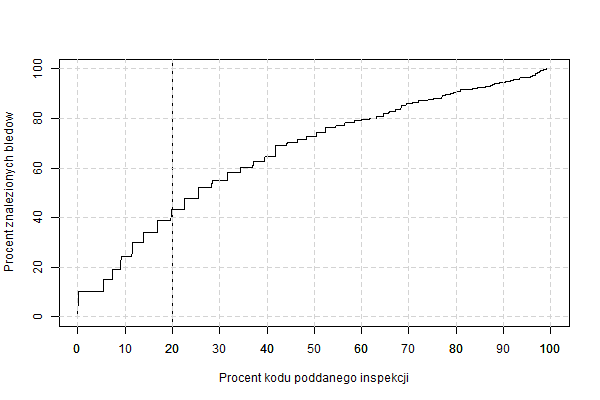
\includegraphics[width=.75\textwidth]{charts/example}
	\label{example-chart}
\end{figure}

Opr�cz okre�lenia wysi�ku, do oceny modeli przyj�to r�wnie� inne miary. \todo{TODO dopisa� jakie i jak si� je liczy, na pewno b�d�: Accuracy, Cohen's kappa coefficient, AUC}


%%%%%%%%%%%%%%%%%%%%%%%%%%%%%%%%%%%%%%%%%%%%%%%%%%%%%%%%%%%%
\chapter{Om�wienie infrastruktury pomiarowej}
\noindent
...

%%%%%%%%%%%%%%%%%%%%%%%%%%%%%%%%%%%%%%%%%%%%%%%%%%%%%%%%%%%% 1
\section{Knime}

\noindent Knime

%%%%%%%%%%%%%%%%%%%%%%%%%%%%%%%%%%%%%%%%%%%%%%%%%%%%%%%%%%%%%%%%%%%%%%%%%%%%%%%%%%%%%%%%%% 2
\subsection{DePress}
\label{depress}

\noindent


%%%%%%%%%%%%%%%%%%%%%%%%%%%%%%%%%%%%%%%%%%%%%%%%%%%%%%%%%%%% 1
\section{Weka}

\noindent Weka







%%%%%%%%%%%%%%%%%%%%%%%%%%%%%%%%%%%%%%%%%%%%%%%%%%%%%%%%%%%% 1
\section{AstCompare (roboczo)}

\noindent AstCompare plugin

%%%%%%%%%%%%%%%%%%%%%%%%%%%%%%%%%%%%%%%%%%%%%%%%%%%%%%%%%%%%%%%%%%%%%%%%%%%%%%%%%%%%%%%%%% 2
\subsection{Wymagania}

\noindent



%%%%%%%%%%%%%%%%%%%%%%%%%%%%%%%%%%%%%%%%%%%%%%%%%%%%%%%%%%%%%%%%%%%%%%%%%%%%%%%%%%%%%%%%%% 2
\subsection{Implementacja}

\noindent



%%%%%%%%%%%%%%%%%%%%%%%%%%%%%%%%%%%%%%%%%%%%%%%%%%%%%%%%%%%%%%%%%%%%%%%%%%%%%%%%%%%%%%%%%% 2
\subsection{Testowanie i gromadzenie danych}

\noindent Metryki zapocz�tkowane przez autor�w i zaimplementowane przez poprzednika (Piotr Mitka \cite{brak_refa}):
\begin{itemize}
	\item allMethodHistories
	\item methodHistories
	\item authors
	\item stmtAdded
	\item maxStmtAdded
	\item avgStmtAdded
	\item stmtUpdated
	\item maxsSmtUpdated
	\item avgStmtUpdated
	\item stmtDeleted
	\item maxStmtDeleted
	\item avgStmtDeleted
	\item stmtParentChanged
	\item churn
	\item maxChurn
	\item avgChurn
	\item decl
	\item cond
\end{itemize}

Metryki dodane przeze mnie:
\begin{itemize}
	\item elseAdded
	\item elseDeleted
	\item loopsAdded
	\item loopsUpdated
	\item loopsDeleted
	\item variablesAdded
	\item variablesUpdated
	\item variablesDeleted
	\item assigmentsAdded
	\item assigmentsUpdated
	\item assigmentsDeleted
	\item returnsAdded
	\item returnsUpdated
	\item returnsDeleted
	\item nullsAdded
	\item nullsUpdated
	\item nullsDeleted
	\item casesAdded
	\item casesUpdated
	\item casesDeleted
	\item breaksAdded
	\item breaksUpdated
	\item breaksDeleted
	\item objectsAdded
	\item objectsUpdated
	\item objectsDeleted
	\item catchesAdded
	\item catchesUpdated
	\item catchesDeleted
	\item throwsAdded
	\item throwsUpdated
	\item throwsDeleted
\end{itemize}

Dodatkowo zaimplementowano drugie wyj�cie wtyczki z wszystkimi historiami metod (do linkowania b��d�w): commit\_id, nazwa metody, autor, komentarz, data.





%%%%%%%%%%%%%%%%%%%%%%%%%%%%%%%%%%%%%%%%%%%%%%%%%%%%%%%%%%%%%%%%%%%%%%%%%%%%%%%%%%%%%%%%%% 2
\subsection{Om�wienie zebranych danych pomiarowych}

\noindent



%%%%%%%%%%%%%%%%%%%%%%%%%%%%%%%%%%%%%%%%%%%%%%%%%%%%%%%%%%%%%%%%%%%%%%%%%%%%%%%%%%%%%%%%%%%%%%%%%%%%%%%%%%%%%%%%%%%%%%%% 3
\subsubsection{Wymagania dla repozytorium metryk}

\noindent



%%%%%%%%%%%%%%%%%%%%%%%%%%%%%%%%%%%%%%%%%%%%%%%%%%%%%%%%%%%%%%%%%%%%%%%%%%%%%%%%%%%%%%%%%%%%%%%%%%%%%%%%%%%%%%%%%%%%%%%% 3
\subsubsection{Struktura danych i zawarto�� zbioru}

\noindent



%%%%%%%%%%%%%%%%%%%%%%%%%%%%%%%%%%%%%%%%%%%%%%%%%%%%%%%%%%%%
\chapter{Modele predykcji i ich ewaluacja}
\noindent
Wykorzystanie RandomForest \cite{hata2012bug, kamei2010revisiting, lessmann2008benchmarking, liaw2002classification, mende2010effort}

Udzia� \% metod z b��dami jest niewielki --- modele predykcji maj� tendencj� do wskazywania wszystkich jako 0, bo ma�o FP --- logistic regression tak mia�o w \cite{hata2012bug}.

Walidacja modelu przez 10-fold cross validation oraz przez testowanie na zbiorze danych z nast�pnego wydania (ang. \textit{release}).

Wykorzystywane algorytmy:
\begin{itemize}
	\item RandomForest
	\item J48
	\item NaiveBayes
	\item Bagging
	\item AdaBoostM1
	\item RacedIncrementalLogitBoost
	\item LMT
	\item BFTree
	\item RandomTree
\end{itemize}


Przebadane projekty:

\begin{figure}[h!]
	\caption{Projekty}
	\centering
	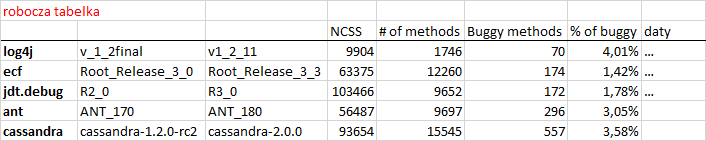
\includegraphics[width=1\textwidth]{img/projekty}
\end{figure}


\begin{figure}[h!]
	\caption{Wyniki}
	\centering
	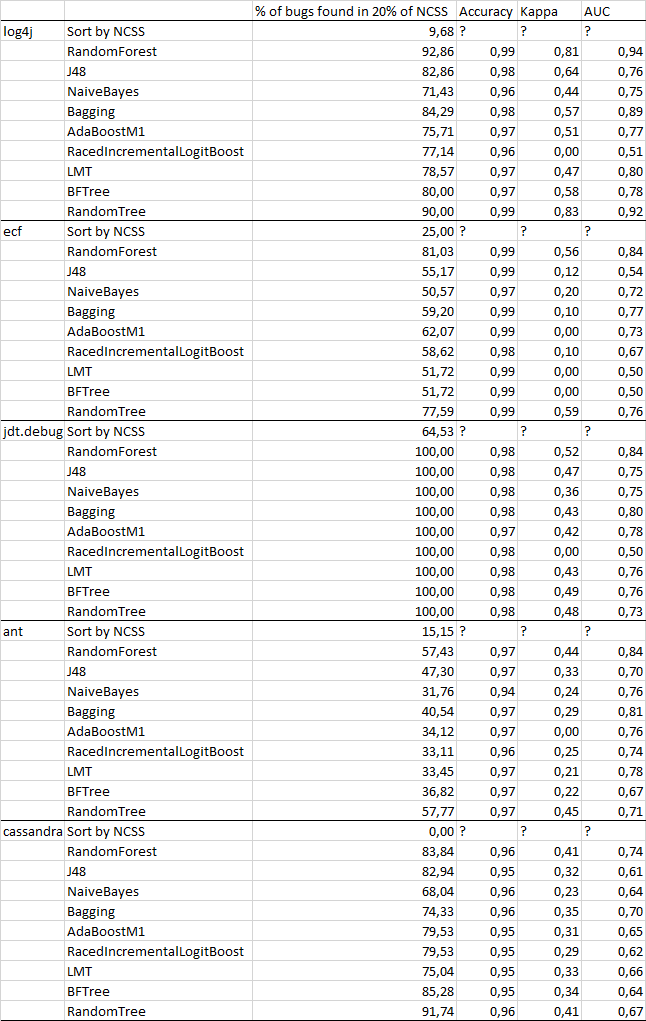
\includegraphics[width=1\textwidth]{img/wyniki}
\end{figure}



\begin{itemize}
	\item NCSS = Non Commenting Source Statements
	\item pierwszy wiersz w wyniku (Sort by NCSS) polega na posortowaniu metod od najmniejszych i sprawdzaniu ich w tej kolejno�ci
	\item kolejne wyniki s� dla modeli opartych na wymienionych wy�ej algorytmach klasyfikacji
	\item wyniki por�wnuj� g��wnie na podstawie efektywno�ci znajdowania b��d�w --- sortuj� wyniki wg prawdopodobie�stwa wyst�pienia b��du w metodzie (algorytmy podaj� zwyci�zc� oraz prawdopodobie�stwa dla 0 i 1), nast�pnie zliczam ile \% b��d�w zostanie odnalezione przy przegl�daniu 20\% kodu w tej kolejno�ci
	\item wyniki w tabeli poni�ej
	\item przyk�adowe wykresy efektywno�ci dla 2 projekt�w poni�ej
	\item na wykresach wybrane 2 projekty kt�re wysz�y najgorzej, w pozosta�ych projektach te krzywe s� jeszcze bardziej strome
\end{itemize}

\begin{figure}[h!]
	\caption{Ant --- Sort by NCSS}
	\centering
	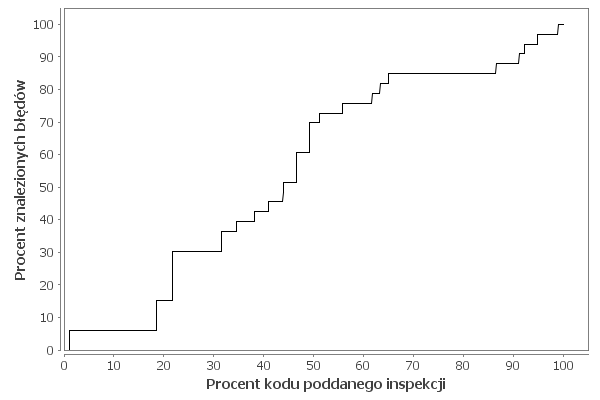
\includegraphics[width=1\textwidth]{charts/ant0}
\end{figure}

\begin{figure}[h!]
	\caption{Ant --- RandomForest}
	\centering
	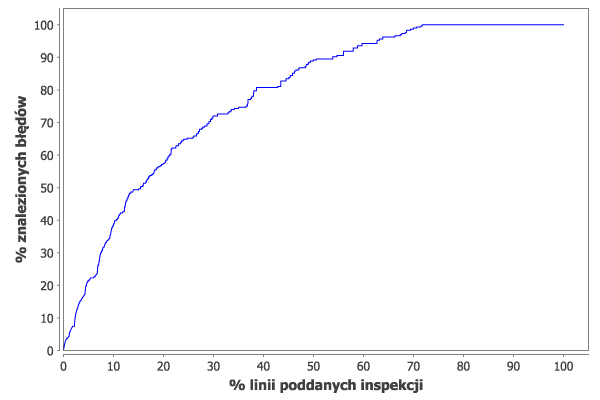
\includegraphics[width=1\textwidth]{charts/ant1}
\end{figure}

\begin{figure}[h!]
	\caption{Ant --- J48}
	\centering
	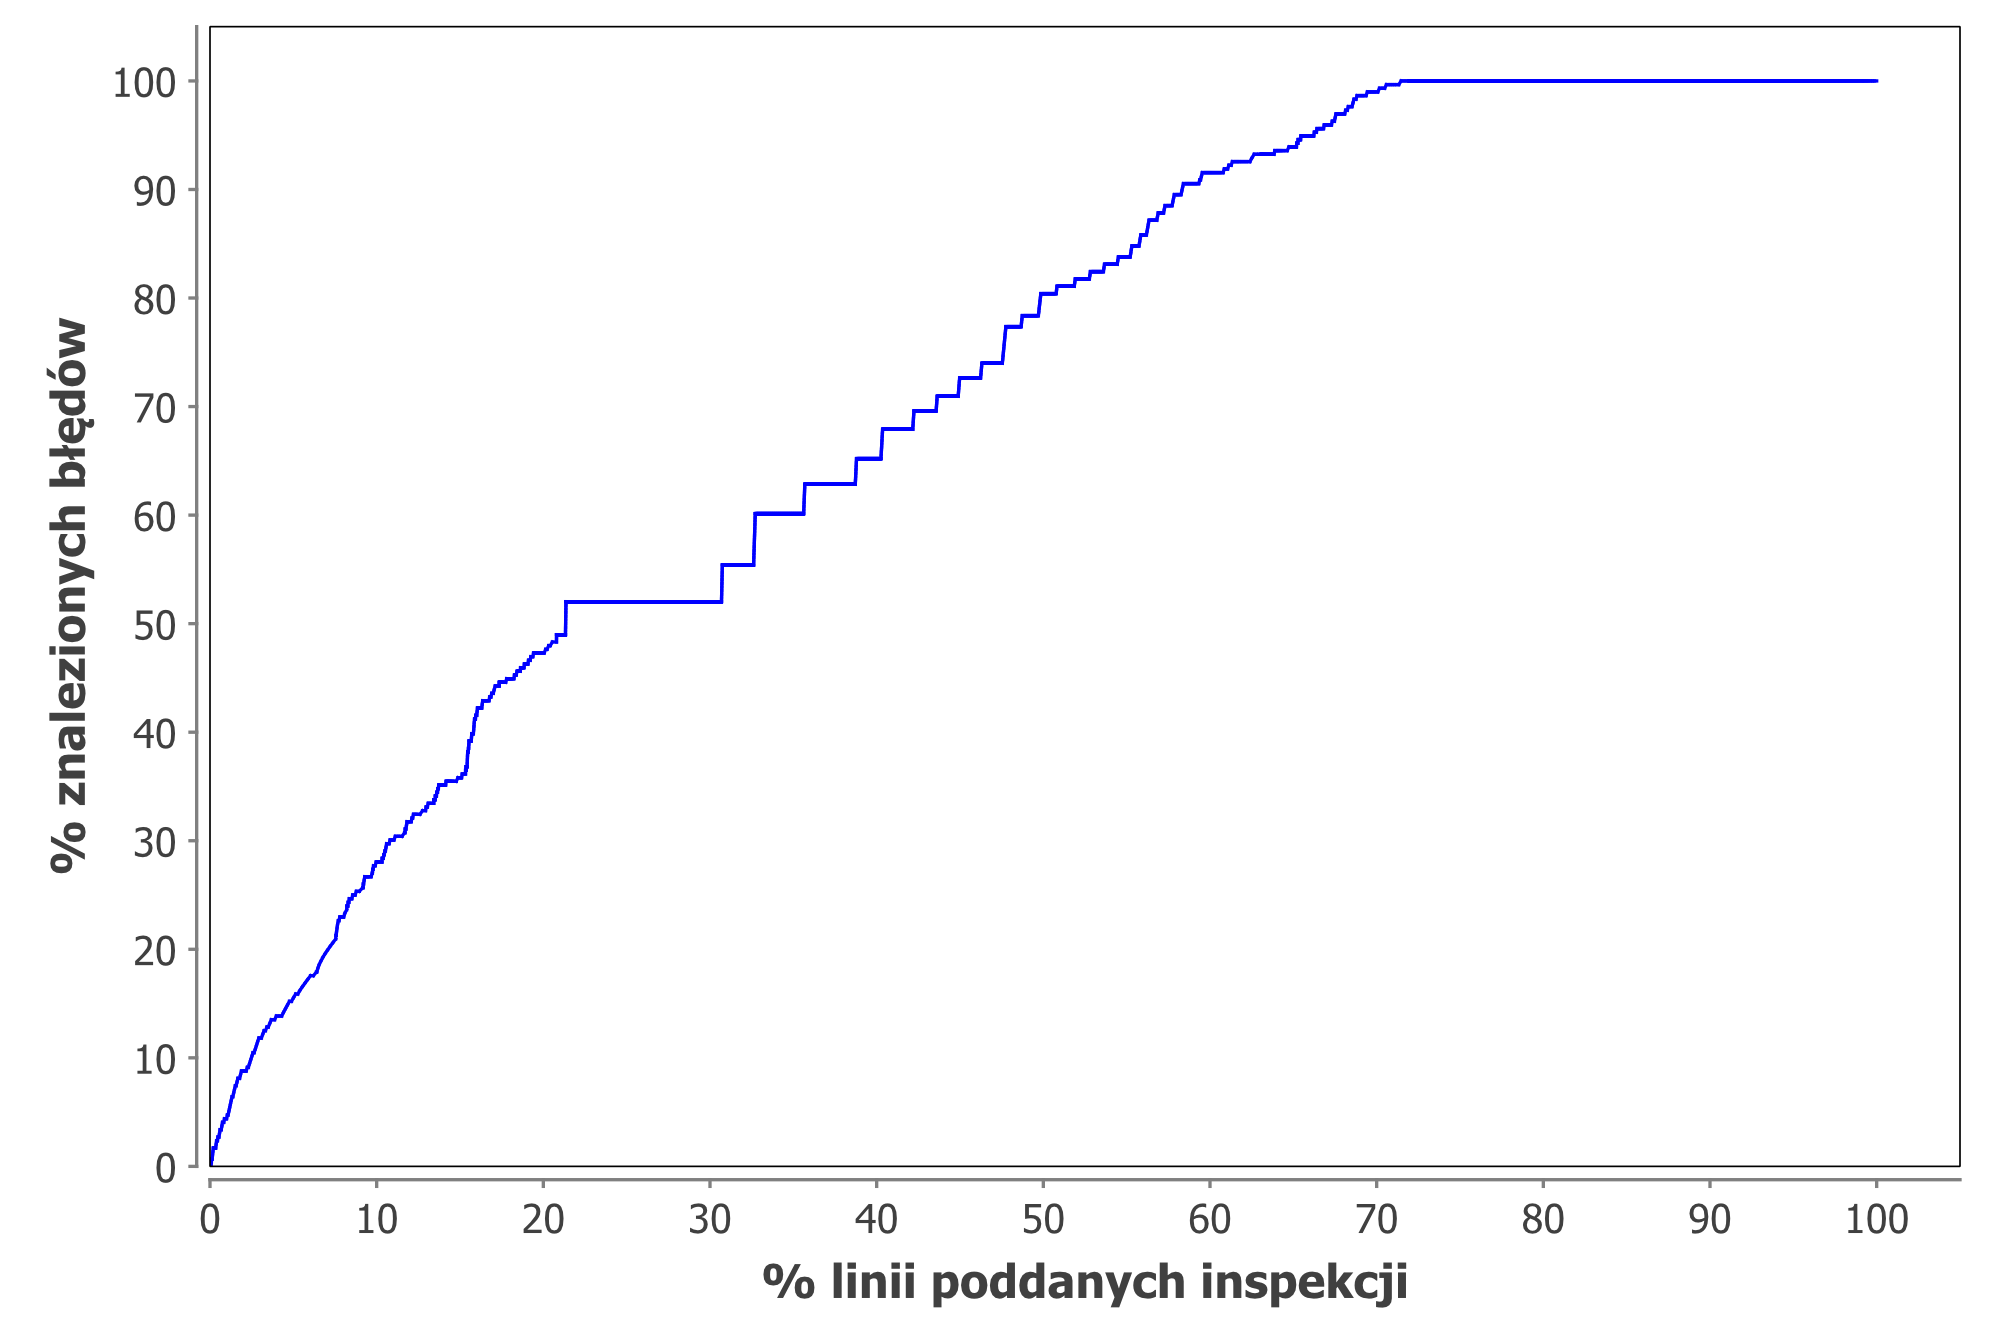
\includegraphics[width=1\textwidth]{charts/ant2}
\end{figure}





\begin{figure}[h!]
	\caption{ECF --- Sort by NCSS}
	\centering
	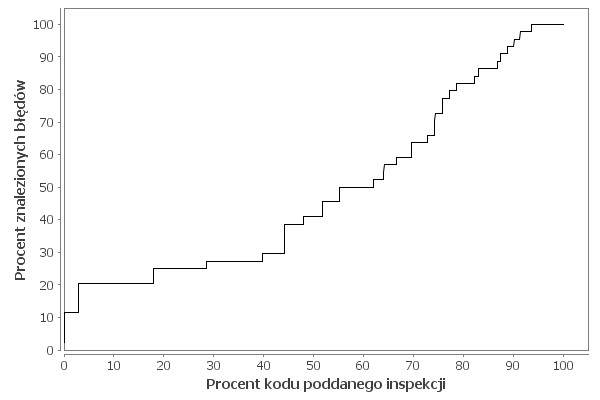
\includegraphics[width=1\textwidth]{charts/ecf0}
\end{figure}

\begin{figure}[h!]
	\caption{ECF --- RandomForest}
	\centering
	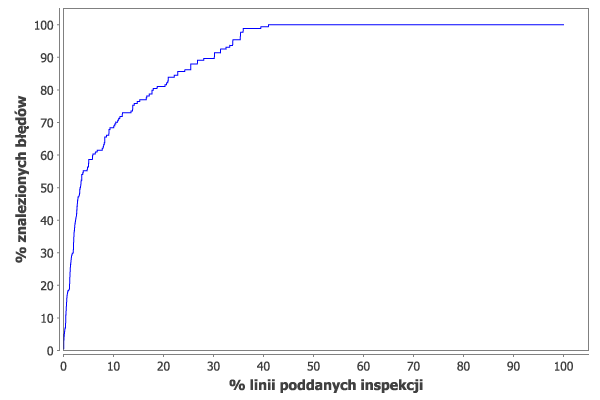
\includegraphics[width=1\textwidth]{charts/ecf1}
\end{figure}

\begin{figure}[h!]
	\caption{ECF --- J48}
	\centering
	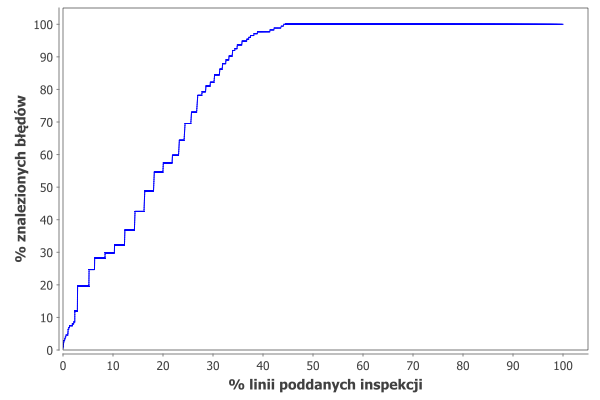
\includegraphics[width=1\textwidth]{charts/ecf2}
\end{figure}


%%%%%%%%%%%%%%%%%%%%%%%%%%%%%%%%%%%%%%%%%%%%%%%%%%%%%%%%%%%% 1
\section{Ocena rozwi�zania}
\noindent

np. Goal-Question-Metric

\begin{itemize}
	\item Stopie� realizacji wymaga� funkcjonalnych
	\item Poprawno�� rozwi�zania (funkcjonowania systemu): weryfikacja (symulacja), testowanie
		\\utworzenie nowego modelu predykcji defekt�w, bazuj�cego na zgromadzonych metrykach w celu weryfikacji przydatno�ci narz�dzi i zgromadzonych metryk
	\item W�a�ciwo�ci (parametry) rozwi�zania
	\item Por�wnanie z innymi rozwi�zaniami
\end{itemize}

%%%%%%%%%%%%%%%%%%%%%%%%%%%%%%%%%%%%%%%%%%%%%%%%%%%%%%%%%%%%
\chapter{Podsumowanie i propozycja dalszych bada�}
\noindent
\begin{itemize}
	\item Wady, zalety, ograniczenia
	\item Wnioski
	\item Zakres zastosowa�, rozw�j i dalsze badania
\end{itemize}

%%%%%%%%%%%%%%%%%%%%%%%%%%%%%%%%%%%%%%%%%%%%%%%%%%%%%%%%%%%%





 
%\listoffigures
%\listoftables

\bibliographystyle{iisthesis}
\bibliography{bibliografia}

%\appendix
%\chapter{Co� dodatkowego}
%\pagestyle{plain}

\end{document}
